\documentclass{book}

\usepackage{ltablex}
\usepackage[colorlinks=true,
    urlcolor=blue,
    linkcolor=red,
    unicode=true]{hyperref}
\usepackage[backend=biber]{biblatex}
\usepackage[utf8]{inputenc}
\usepackage[T1]{fontenc}
\usepackage[main=hindi,russian,english]{babel}
\usepackage{imakeidx}
\usepackage{xcolor}   % Compiler recommended to load package
\usepackage{fontspec} % Compiler recommended to load package
\usepackage{csquotes} % Compiler recommended to load package
\usepackage{xparse}   % Compiler recommended to load package

%
\babelfont[hindi]{rm}{Nirmala UI}
\babelfont[russian]{rm}{Segoe UI}

\makeindex[columns=2, title=वर्णक्रमानुसार सूची, intoc]

\NewDocumentCommand {\ru}{+m}{\foreignlanguage{russian}{#1}}
\NewDocumentCommand {\ruit}{+m}{\foreignlanguage{russian}{\textit{#1}}}
\NewDocumentCommand{\rusmalld}{}{\fontspec{Lucida Calligraphy} \selectfont \textit{g}}

\addbibresource{bibliography.bib}

% Used for tabularx package to put some gap between text and row heights 
\renewcommand{\arraystretch}{1.5}

\title{हिन्दी भाषियों के लिए रूसी अध्यन}
\author{Vinay Pandey}

\includeonly{chapters/intro.tex}

\begin{document}

    \maketitle
    \tableofcontents

    \chapter{रूसी वर्णमाला, उच्चारण, तथा वर्तनी नियम}\label{ch:intro}

  \section{वर्णमाला} \label{sec: intro-alpha-list}
\begin{tabularx}{\linewidth}{ c c c c c X }
    \caption{वर्णमाला}\label{tab: alphabet}  \tabularnewline
    \toprule

    \midrule
    \textbf{बड़ी लिपि} & \textbf{छोटी लिपि} & \textbf{Italics} & \textbf{Big Cursive} & \textbf{Small Cursive}  & \textbf{हिन्दी उच्चारण} \tabularnewline
    \midrule
    \endfirsthead

    \midrule
    \textbf{बड़ी लिपि} & \textbf{छोटी लिपि} & \textbf{Italics} & \textbf{Big Cursive} & \textbf{Small Cursive}  & \textbf{हिन्दी उच्चारण} \tabularnewline
    \midrule
    \endhead

    \midrule
    \multicolumn{5}{r}{\footnotesize{अगले पृष्ट पर जारी}} \tabularnewline
    \endfoot

    \bottomrule
    \multicolumn{5}{r}{\footnotesize{इति तालिका~\ref{tab: alphabet} }} \tabularnewline
    \endlastfoot

    \ru{А} & \ru{а} & \ruit{а} & \ruscursive{А} & \ruscursive{а} & अ \tabularnewline
    \ru{Б} & \ru{б} & \ruit{б} & \ruscursive{Б} & \ruscursive{б} & ब \tabularnewline
    \ru{В} & \ru{в} & \ruit{в} & \ruscursive{В} & \ruscursive{в} & व \tabularnewline
    \ru{Г} & \ru{г} & \ruit{г} & \ruscursive{Г} & \ruscursive{г} & ग \tabularnewline
    \ru{Д} & \ru{д} & \ruit{д} & \ruscursive{Д} & \ruscursive{д} & ड \tabularnewline
    \ru{Е} & \ru{е} & \ruit{е} & \ruscursive{Е} & \ruscursive{е} & येह् \tabularnewline
    \ru{Ё} & \ru{ё} & \ruit{ё} & \ruscursive{Ё} & \ruscursive{ё} & यो \tabularnewline
    \ru{Ж} & \ru{ж} & \ruit{ж} & \ruscursive{Ж} & \ruscursive{ж} & क्ज़, अंग्रेजी भाषा के \textit{tre\underline{asu}re}/\textit{ट्रेज़र} के ज़ कि भांति \tabularnewline
    \ru{З} & \ru{з} & \ruit{з} & \ruscursive{З} & \ruscursive{з} & ज़ \tabularnewline
    \ru{И} & \ru{и} & \ruit{и} & \ruscursive{И} & \ruscursive{и} & इ \tabularnewline
    \ru{Й} & \ru{й} & \ruit{й} & \ruscursive{Й} & \ruscursive{й} & य \tabularnewline
    \ru{К} & \ru{к} & \ruit{к} & \ruscursive{К} & \ruscursive{к} & क \tabularnewline
    \ru{Л} & \ru{л} & \ruit{л} & \ruscursive{Л} & \ruscursive{л} & ल \tabularnewline
    \ru{М} & \ru{м} & \ruit{м} & \ruscursive{М} & \ruscursive{м} & म \tabularnewline
    \ru{Н} & \ru{н} & \ruit{н} & \ruscursive{Н} & \ruscursive{н} & ह \tabularnewline
    \ru{О} & \ru{о} & \ruit{о} & \ruscursive{О} & \ruscursive{о} & ओ \tabularnewline
    \ru{П} & \ru{п} & \ruit{п} & \ruscursive{П} & \ruscursive{п} & प \tabularnewline
    \ru{Р} & \ru{р} & \ruit{р} & \ruscursive{Р} & \ruscursive{р} & र \tabularnewline
    \ru{С} & \ru{с} & \ruit{с} & \ruscursive{С} & \ruscursive{с} & स \tabularnewline
    \ru{Т} & \ru{т} & \ruit{т} & \ruscursive{Т} & \ruscursive{т} & ट \tabularnewline
    \ru{У} & \ru{у} & \ruit{у} & \ruscursive{У} & \ruscursive{у} & उ \tabularnewline
    \ru{Ф} & \ru{ф} & \ruit{ф} & \ruscursive{Ф} & \ruscursive{ф} & फ \tabularnewline
    \ru{Х} & \ru{х} & \ruit{х} & \ruscursive{Х} & \ruscursive{х} & ख \tabularnewline
    \ru{Ц} & \ru{ц} & \ruit{ц} & \ruscursive{Ц} & \ruscursive{ц} & त्स \tabularnewline
    \ru{Ч} & \ru{ч} & \ruit{ч} & \ruscursive{Ч} & \ruscursive{ч} & च \tabularnewline
    \ru{Ш} & \ru{ш} & \ruit{ш} & \ruscursive{Ш} & \ruscursive{ш} & श \tabularnewline
    \ru{Щ} & \ru{щ} & \ruit{щ} & \ruscursive{Щ} & \ruscursive{щ} & ष \tabularnewline
    \ru{Ъ} & \ru{ъ} & \ruit{ъ} & \ruscursive{Ъ} & \ruscursive{ъ} & ~\ref{subsubsec:alpha-pronounce-special-char-hard} भाग देखिए \tabularnewline
    \ru{Ы} & \ru{ы} & \ruit{ы} & \ruscursive{Ы} & \ruscursive{ы} & ~\ref{subsubsec:alpha-pronounce-special-char-oui} भाग देखिए \tabularnewline
    \ru{Ь} & \ru{ь} & \ruit{ь} & \ruscursive{Ь} & \ruscursive{ь} & \index{\ru{ь}|see {\ru{мякий знак}}}~\ref{subsubsec:alpha-pronounce-special-char-soft} भाग देखिए \tabularnewline
    \ru{Э} & \ru{э} & \ruit{э} & \ruscursive{Э} & \ruscursive{э} & ए \tabularnewline
    \ru{Ю} & \ru{ю} & \ruit{ю} & \ruscursive{Ю} & \ruscursive{ю} & यू \tabularnewline
    \ru{Я} & \ru{я} & \ruit{я} & \ruscursive{Я} & \ruscursive{я} & या
\end{tabularx}

  \section{उच्चारण}\label{sec:intro-pronounce}\index{उच्चारण}
हिन्दी की तरह, रूसी भाषा में भी अधिकतर जैसा लिखते हैं वैसा ही बोलते हैं। परंतु इसमे कुछ अपवाद भी हैं, प्रधानत:
\begin{itemize}
    \item \ru{его} को लिखते \textit{यगो} हैं परंतु बोलते \textit{यवो} हैं
    \item \ru{--ого} को लिखते \textit{ओगो} हैं परंतु बोलते \textit{ओवो} हैं, यह शब्द प्राय: उपसर्ग (suffix) में होता है।
    \item \ru{что} को लिखते \textit{च्तो} हैं पर पढ़ते ष्तो हैं। इसी तरह बहुत ऐसे शब्द हैं जहां \ru{ч} का उच्चारण ष कि तरह होता है।
\end{itemize}

रूसी शब्दों के उच्चारण मे यह बहुत महत्वपूर्ण है कि शब्द के किस भाग पर बल दिया जा रहा है, उदाहरत:
\begin{itemize}
    \item \ru{ст\'оит} [उच्चारण: स्तोइत; धातु: \ru{стоять}] का अर्थ किसी वस्तु, व्यक्ति, अथवा जन्तु के खड़े होने से
    है। \par उदाहरण के लिए: \ru{он стоит там} $\rightarrow$ वह वहाँ खड़ा है।
    \item \ru{сто\'ит} [उच्चारण: स्तईत; धातु: \ru{стоить}] का अर्थ पैसा अथवा किसी वस्तु का मूल्य होता है| \par उदाहरण के लिए: \ru{сколько стоит} $\rightarrow$ कितना मूल्य है।
\end{itemize}

इसी प्रकार~\cite{levine2009}:
\begin{itemize}
    \item \ru{мук\'а}\index{\ru{мук\'а}} [उच्चारण: मुका] का अर्थ आटा है, और,
    \item \ru{м\'ука}\index{\ru{м\'ука}} [उच्चारण: मूका] का अर्थ दु:ख, दर्द, अथवा प्रताड़ना है।
\end{itemize}

इसी कारण कई पुस्तकों में शब्द के जिस अक्षर पर बल देना हो, उसे accent {\color{blue} {\large $\left( \acute{\,}\, \right)$}} से चिन्हित किया गया होता है। % Latex -> \, => small space in maths mode

\subsection{\sru{ъ}, \sru{ь}, तथा \sru{ы} का उच्चारण}\label{subsec:alpha-pronounce-special-char}

\ru{ъ} और \sru{ь} उच्चारण के अक्षर हैं और इनका अलग से उच्चारण नहीं होता है, यह दोनों अक्षर जिस शब्द के आगे लगते हैं उन पर कम या ज़्यादा बल देना होता
है। इन्ही कारणों से इन्हे \ru{твёрди знак}, \ru{твёрди} = कठोर, और \ru{мякий знак}, \ru{мякий} = कोमल, \ru{знак} = चिन्ह कहा जाता है।

\subsubsection{\sru{ъ}: \sru{твёрди знак}: [त्वयोरदी ज़्नाक]}\label{subsubsec:alpha-pronounce-special-char-hard}\index{\ru{твёрди знак}}
इसे कठोर चिन्ह कहते हैं, इसका कोई अलग से उच्चारण नहीं है, यह जिस अक्षर के आगे लगता है उस पर बल देना होता है। यह संस्कृत भाषा के s चिन्ह कि तरह है। उदाहरण के लिए:
\begin{itemize}
    \item \ru{съ\'езд}\index{\ru{съезд}} $\rightarrow$
    \item \ru{съ\'есть}\index{\ru{съесть}} $\rightarrow$
    \item \ru{объявить}\index{\ru{объявить}} $\rightarrow$
    \item \ru{объëму}\index{\ru{объëму}} $\rightarrow$
    \item \ru{съëмки}\index{\ru{съëмки}} $\rightarrow$
\end{itemize}

यह अक्षर 1917 से पहले लगभग हर शब्द के अंत मे लगता था, परंतु 1917 के क्रांतिकारी तख्तापलट के पशच्यात इसे खतम कर दिया गया। इस अक्षर का प्रयोग दो शब्दों को विभाजित
करने के लिए भी होता था~\cite{guzeva2020}।

%% Insert diagram here

\subsubsection{\sru{ь}: \sru{мякий знак}: [म्याकि ज़्नाक]}\label{subsubsec:alpha-pronounce-special-char-soft}\index{\ru{мякий знак}}
यह कोमल उच्चारण का चिन्ह है, हिन्दी/संस्कृत के हलंत की तरह उच्चारण होना चाहिए, परंतु कई बार ये ऐसे अक्षरों के आगे भी लग जाता है जिनके आगे प्राय: हिन्दी या संस्कृत में
हलंत नहीं लगाते। यह चिन्ह जिस अक्षर के आगे लगता है, उच्चारण के समय के समय जिह्वा ऊपर के आगे के दांतों को छू रही होती है। जैसे \ru{брать} [ब्रात] (भ्राता/भाई) में `त्'
को उच्चारित करने के लिए `त' बोलते समय जिह्वा ऊपर के मुख के सामने के दांतों को पीछे कि तरफ से छूती है। इसे \ref{fig:intro-pronounce-soft} में दर्शाया गया है।

\begin{figure}
    \label{fig:intro-pronounce-soft}

    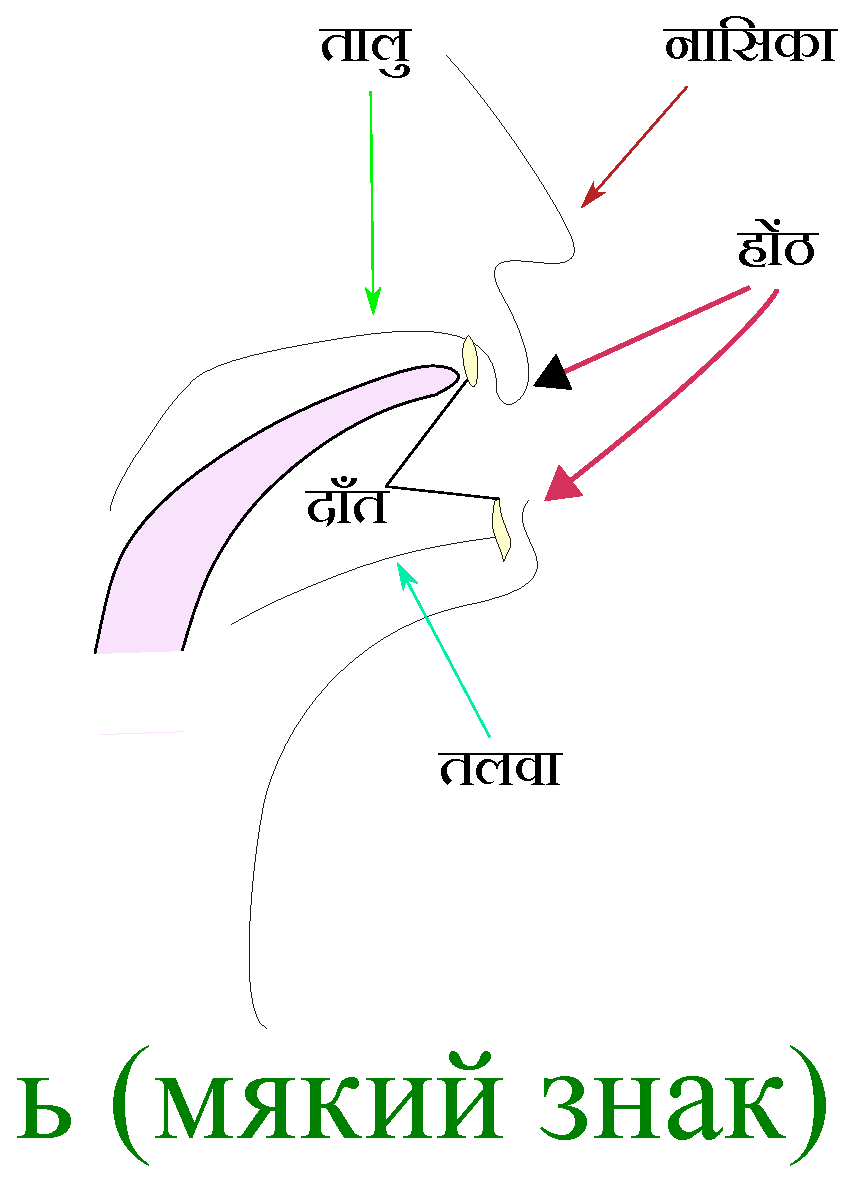
\includegraphics[scale=0.35]{graphics/pronounce-soft}
    \caption{\ru{ь} का उच्चारण}

\end{figure}

\subsubsection{\sru{ы}}\label{subsubsec:alpha-pronounce-special-char-oui}\index{\ru{ы}}
इसे `ऋ' अक्षर में अगर `र' की ध्वनि निकाल दी जाए, और अंत के `ई' के जैसे उच्चारित करते हैं। संस्कृत भाषा में
ऐसे अक्षरों को जिह्वामूलीय अक्षर कहते हैं, जहां ध्वनि जिव्हा की जड़ से निकलती है, और जिह्वा स्वय: मुँह के
बीच में रहती है, न ऊपर न नीचे के दांतों को छूती ह~\cite{macdonald1926}। इसे~\ref{fig:intro-pronounce-oui} में दर्शाया गया है।
उच्चारण के लिए \href{https://www .youtube .com/watch?v=s6asiEL1f8U}{यह विडिओ}~\cite{kovalenko2015} देखिए।
\begin{figure}
    \label{fig:intro-pronounce-oui}
    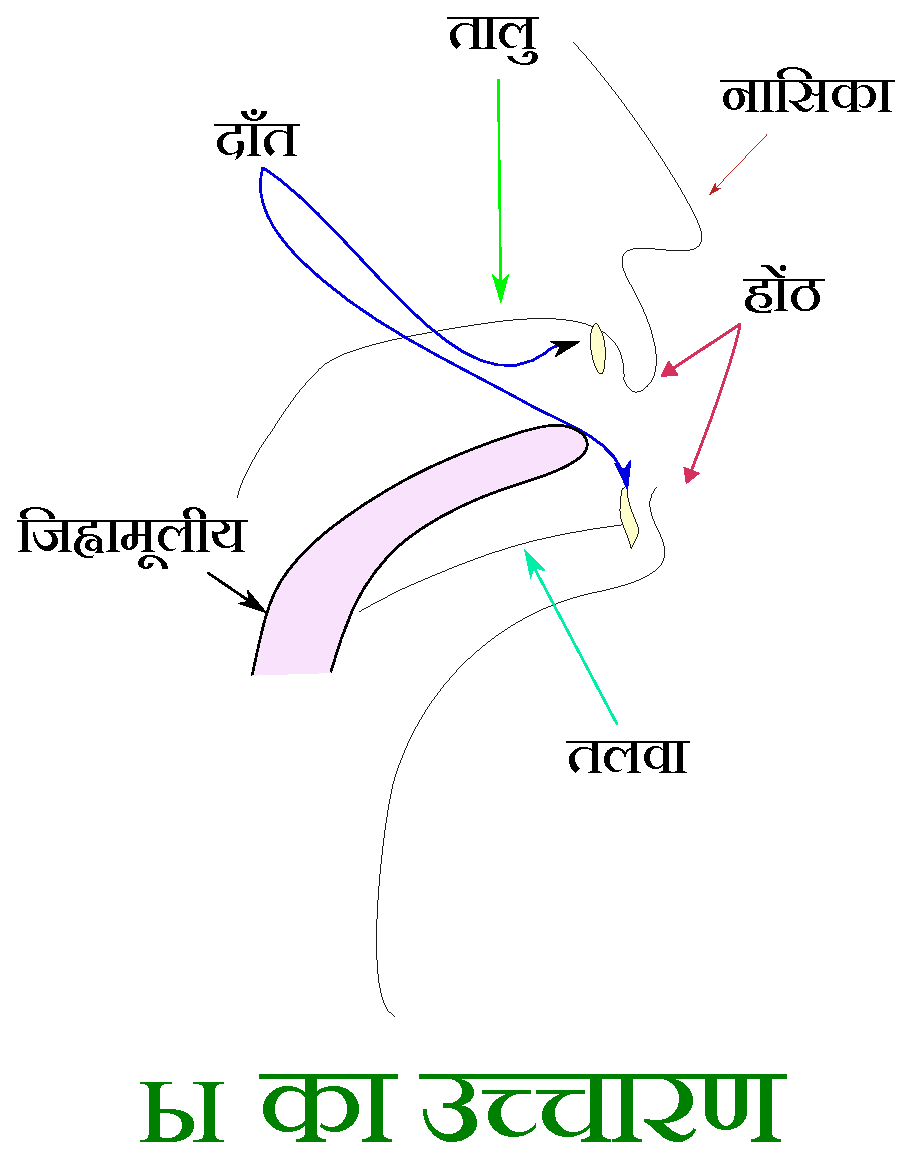
\includegraphics[scale=0.35]{graphics/pronounce-oui}
    \caption{\ru{ы} का उच्चारण}
\end{figure}

  \section{वर्तनी के नियम (Spelling Rules)}\label{sec:intro-spelling}
रूसी भाषा के अक्षरों को लिखते समय निम्नलिखित नियम ध्यान रखिए, इनका विवरण आवश्यकतानुसार आगे भी दिया जाएगा। इन नियमों
को स्मरित रखना अत्यधिक आवश्यक है, क्योंकि यह नियम आगे कारक~\ref{ch:cases} में प्रयोग होंगे, जो हिन्दी व्याकरण कि
तरह, रूसी भाषा में महत्व रखते हैं।~\cite{levine2009, robin2012, wade2011}

\subsection{\sru{К}, \sru{Г}, \sru{Х}}\label{subsec:alpha-spelling-k-g-h}
\begin{enumerate}
  \item इनके आगे हमेशा \ru{-у} (ऊ) लगेगा, कभी भी \ru{-ю} (यू) नहीं
  \item इनके आगे हमेशा \ru{-ы} लगेगा, कभी भी \ru{-и} (ई) नहीं
  \item इनके आगे हमेशा \ru{-а} (आ) लगेगा, कभी भी \ru{-я} (या) नहीं
\end{enumerate}

\subsection{\sru{Ц}}\label{subsec:alpha-spelling-ts}
\begin{enumerate}
  \item इनके आगे हमेशा \ru{-у} (ऊ) लगेगा, कभी भी \ru{-ю} (यू) नहीं
  \item इनके आगे हमेशा \ru{-ы} लगेगा, कभी भी \ru{-и} (ई) नहीं
  \item इसके आगे हमेशा सबल \ru{-\'е} (ये) लगेगा, कभी भी साधारण \ru{-о} (ओ) नहीं
\end{enumerate}

\subsection{\sru{Ж}, \sru{Ч}, \sru{Ш}, \sru{Щ}}\label{subsec:alpha-spelling-zh-ch-sh-scsh-ts}
\begin{enumerate}
  \item इनके आगे हमेशा \ru{-у} (ऊ) लगेगा, कभी भी \ru{-ю} (यू) नहीं
  \item इनके आगे हमेशा \ru{-ы} लगेगा, कभी भी \ru{-и} (ई) नहीं
  \item इनके आगे हमेशा \ru{-а} (आ) लगेगा, कभी भी \ru{-я} (या) नहीं
  \item इनके आगे हमेशा सबल \ru{-\'е} (ये) लगेगा, कभी भी साधारण \ru{-о} (ओ) नहीं
\end{enumerate}

    \chapter{संज्ञा}\label{ch: noun}

\section{लिंग}\label{sec:noun-gender}
हिन्दी कि तरह रूसी भाषा में भी संज्ञा के तीन लिंग [род] \index{род} होते हैं :

स्त्रीलिंग\index{स्त्रीलिंग}  Женский род [जेन्सकीय रोद]
पुलिंग\index{पुलिंग} Мужской род [मूज़कोय रोद]
नपुंसकलिंग\index{नपुंसकलिंग} Средний род [स्रेदनीय रोद]

सामान्यत: स्त्रीलिंग शब्द \ru{-а} (आ), \ru{-ь} (\ru{мякий знак}),  अथवा \ru{-я} (या)  से अंत होते हैं, नपुंसकलिंग  प्राय: \ru{-о} (ओ) अथवा 
\ru{-е} (ये) से अंत होते हैं, पुलिंग शब्द बाकी किसी भी अक्षर से अंत हो सकते हैं। यह ध्यान रखिए कि इस नियम के बहुत अपवाद भी हैं, ऐसे अपवादों का उल्लेख 
आवश्यकतानुसार किया जाएगा। रूसी भाषा ने कई भाषाओं के शब्दों को आत्मसात किया है, ऐसे शब्दों का लिंग निर्धारण उनकी मूल भाषा के अनुरूप किया जाता है।


    \chapter{सर्वनाम}\label{ch: pronoun}
    \chapter{काल}\label{ch: tenses}
    \chapter{कारक}\label{ch:cases}

हिन्दी मे कारक कि तरह रूसी भाषा में भी कारक होते हैं। इन्हे संज्ञा, सर्वनाम, विशेषण इत्यादि में प्रयोग करते हैं।


\section{कर्ता कारक} \label{sec:nominative-case}


\section{कर्म कारक} \label{sec:accusative-case}


\section{करण कारक} \label{sec:instrumental-case}


\section{संबंध कारक}  \label{sec:prepositional-case}


\section{संप्रदान कारक}  \label{sec:dative-case}


\section{अधिकरण कारक} \label{sec:genitive-case}


\section{अपादान कारक} \label{sec:ablative-case}

    \printbibliography
    \printindex
\end{document}